\documentclass[11pt,twocolumn,oneside,openany,headings=optiontotoc,11pt,numbers=noenddot]{article}

\usepackage[a4paper]{geometry}
\usepackage[utf8]{inputenc}
\usepackage[T1]{fontenc}
\usepackage{lmodern}
\usepackage[ngerman]{babel}
\usepackage{ngerman}

\usepackage[onehalfspacing]{setspace}

\usepackage{fancyhdr}
\usepackage{fancybox}

\usepackage{rotating}
\usepackage{varwidth}

%Struktogramme
\usepackage[german,curves]{struktex}

\usepackage{pdflscape}
\usepackage{changepage}
\usepackage{graphicx}
\usepackage[bottom]{footmisc}
\usepackage{transparent}
\usepackage{graphbox}
\graphicspath{
	{Pics/PDFs/}
	{Pics/JPGs/}
	{Pics/PNGs/}
}
\usepackage{caption}
\usepackage{wrapfig}
\usepackage{marginnote}
\usepackage{tabularx}
\usepackage{dashrule}
\usepackage{soulutf8}
\usepackage{hhline}
%arydshln suppresses vertical lines in table
%\usepackage{arydshln}
\usepackage{multirow}
\usepackage{enumerate}
\usepackage[hidelinks]{hyperref}
\usepackage{listings}

\usepackage[table]{xcolor}
\usepackage{array}
\usepackage{enumitem,amssymb,amsmath}
\usepackage{interval}
\usepackage{cancel}
\usepackage{stmaryrd}
\usepackage{wasysym}
\usepackage{polynom}
\usepackage{diagbox}
\usepackage{dashrule}
\usepackage{framed}
\usepackage{mdframed}
\usepackage{karnaugh-map}
\usepackage{pdfpages}

\usepackage{blindtext}

\usepackage{eso-pic}

\usepackage{amssymb}
\usepackage{eurosym}

\usepackage[pages=some]{background}
\pagestyle{headings}
\renewcommand{\headrulewidth}{0.2pt}
\renewcommand{\footrulewidth}{0.2pt}
\newcommand*{\underdownarrow}[2]{\ensuremath{\underset{\overset{\Big\downarrow}{#2}}{#1}}}
\setlength{\fboxsep}{5pt}
\newcommand{\explainBelow}[3]{\underbrace{#1}_{\parbox{\widthof{#3}}{\footnotesize\raggedright #2}}}
\newcommand{\explainAbove}[3]{\overbrace{#1}^{\parbox{\widthof{#3}}{\footnotesize\raggedright #2}}}
\newcommand\footnoteref[1]{\protected@xdef\@thefnmark{\ref{#1}}\@footnotemark}


% Codestyle defined
\definecolor{codegreen}{rgb}{0,0.6,0}
\definecolor{codegray}{rgb}{0.5,0.5,0.5}
\definecolor{codepurple}{rgb}{0.58,0,0.82}
\definecolor{backcolour}{rgb}{0.95,0.95,0.92}
\definecolor{deepgreen}{rgb}{0,0.5,0}
\definecolor{darkblue}{rgb}{0,0,0.65}
\definecolor{mauve}{rgb}{0.40, 0.19,0.28}
\colorlet{exceptioncolour}{yellow!50!red}
\colorlet{commandcolour}{blue!60!black}
\colorlet{numpycolour}{blue!60!green}
\colorlet{specmethodcolour}{violet}

%Neue Spaltendefinition
\newcolumntype{L}[1]{>{\raggedright\let\newline\\\arraybackslash\hspace{0pt}}m{#1}}
\newcolumntype{M}{>{\centering\arraybackslash}X}
\newcommand{\cmnt}[1]{\ignorespaces}
%Textausrichtung ändern
\newcommand\tabrotate[1]{\rotatebox{90}{\raggedright#1\hspace{\tabcolsep}}}

%Intervall-Konfig
\intervalconfig {
	soft open fences
}

%Bash
\lstdefinestyle{BashInputStyle}{
	language=bash,
	basicstyle=\small\sffamily,
	backgroundcolor=\color{backcolour},
	columns=fullflexible,
	backgroundcolor=\color{backcolour},
	breaklines=true,
}
%Java
\lstdefinestyle{JavaInputStyle}{
	language=Java,
	backgroundcolor=\color{backcolour},
	aboveskip=1mm,
	belowskip=1mm,
	showstringspaces=false,
	columns=flexible,
	basicstyle={\footnotesize\ttfamily},
	numberstyle={\tiny},
	numbers=none,
	keywordstyle=\color{purple},,
	commentstyle=\color{deepgreen},
	stringstyle=\color{blue},
	emph={out},
	emphstyle=\color{darkblue},
	emph={[2]rand},
	emphstyle=[2]\color{specmethodcolour},
	breaklines=true,
	breakatwhitespace=true,
	tabsize=2,
}
%Python
\lstdefinestyle{PythonInputStyle}{
	language=Python,
	alsoletter={1234567890},
	aboveskip=1ex,
	basicstyle=\footnotesize,
	breaklines=true,
	breakatwhitespace= true,
	backgroundcolor=\color{backcolour},
	commentstyle=\color{red},
	otherkeywords={\ , \}, \{, \&,\|},
	emph={and,break,class,continue,def,yield,del,elif,else,%
		except,exec,finally,for,from,global,if,import,in,%
		lambda,not,or,pass,print,raise,return,try,while,assert},
	emphstyle=\color{exceptioncolour},
	emph={[2]True,False,None,min},
	emphstyle=[2]\color{specmethodcolour},
	emph={[3]object,type,isinstance,copy,deepcopy,zip,enumerate,reversed,list,len,dict,tuple,xrange,append,execfile,real,imag,reduce,str,repr},
	emphstyle=[3]\color{commandcolour},
	emph={[4]ode, fsolve, sqrt, exp, sin, cos, arccos, pi,  array, norm, solve, dot, arange, , isscalar, max, sum, flatten, shape, reshape, find, any, all, abs, plot, linspace, legend, quad, polyval,polyfit, hstack, concatenate,vstack,column_stack,empty,zeros,ones,rand,vander,grid,pcolor,eig,eigs,eigvals,svd,qr,tan,det,logspace,roll,mean,cumsum,cumprod,diff,vectorize,lstsq,cla,eye,xlabel,ylabel,squeeze},
	emphstyle=[4]\color{numpycolour},
	emph={[5]__init__,__add__,__mul__,__div__,__sub__,__call__,__getitem__,__setitem__,__eq__,__ne__,__nonzero__,__rmul__,__radd__,__repr__,__str__,__get__,__truediv__,__pow__,__name__,__future__,__all__},
	emphstyle=[5]\color{specmethodcolour},
	emph={[6]assert,range,yield},
	emphstyle=[6]\color{specmethodcolour}\bfseries,
	emph={[7]Exception,NameError,IndexError,SyntaxError,TypeError,ValueError,OverflowError,ZeroDivisionError,KeyboardInterrupt},
	emphstyle=[7]\color{specmethodcolour}\bfseries,
	emph={[8]taster,send,sendMail,capture,check,noMsg,go,move,switch,humTem,ventilate,buzz},
	emphstyle=[8]\color{blue},
	keywordstyle=\color{blue}\bfseries,
	rulecolor=\color{black!40},
	showstringspaces=false,
	stringstyle=\color{deepgreen}
}

\lstset{literate=%
	{Ö}{{\"O}}1
	{Ä}{{\"A}}1
	{Ü}{{\"U}}1
	{ß}{{\ss}}1
	{ü}{{\"u}}1
	{ä}{{\"a}}1
	{ö}{{\"o}}1
}

% Neue Klassenarbeits-Umgebung
\newenvironment{worksheet}[3]
% Begin-Bereich
{
	\newpage
	\sffamily
	\setcounter{page}{1}
	\ClearShipoutPicture
	\AddToShipoutPicture{
		\put(55,761){{
				\mbox{\parbox{385\unitlength}{\tiny \color{codegray}BBS I Mainz, #1 \newline #2
						\newline #3
					}
				}
			}
		}
		\put(455,761){{
				\mbox{\hspace{0.3cm}
\includegraphics[width=0.2\textwidth]{../../logo.pdf}}
			}
		}
	}
}
% End-Bereich
{
	\clearpage
	\ClearShipoutPicture
}

\setlength{\columnsep}{3em}
\setlength{\columnseprule}{0.5pt}

\geometry{left=1.50cm,right=1.50cm,top=3.00cm,bottom=1.00cm,includeheadfoot}
\pagenumbering{gobble}
\pagestyle{empty}

\begin{document}
	\begin{worksheet}{Mathematik}{Lernabschnitt: Differenzialrechnung}{Kurvendiskussion - Extremstellen}
		\subsubsection*{Was wir bei ganzrationalen Funktionen schon bestimmen können}
		\begin{itemize}[label=-]
			\item Symmetrie
			\item Verhalten für große x-Beträge
			\item y-Achsenabschnitt
			\item Nullstellen
		\end{itemize}
		\subsubsection*{\underline{Begrifflichkeiten}}
		\textbf{relatives Maximum} bezeichnet den \(y\)-Wert des Punktes, der in direkter Umgebung zu der Stelle \(x_{max}\) am \textbf{\underline{größten}} ist.\\
		\par\noindent
		\textbf{relatives Minimum} bezeichnet den \(y\)-Wert des Punktes, der in direkter Umgebung zu der Stelle \(x_{min}\) am \underline{\textbf{kleinsten}} ist.\\
		\par\noindent
		\textbf{Extremstelle} bezeichnet die Stelle \(x_{max}/x_{min}\), an der der \textbf{\underline{größte/kleinste}} \(y\)-Wert in direkter Umgebung erreicht wird.\\
		\par\noindent
		\textbf{Extrempunkt} wird ein Punkt \(E(x_E|y_E)\) genannt, der entweder \underline{relatives Maximum} oder \underline{relatives Minimum} ist.\\
		\par\noindent
		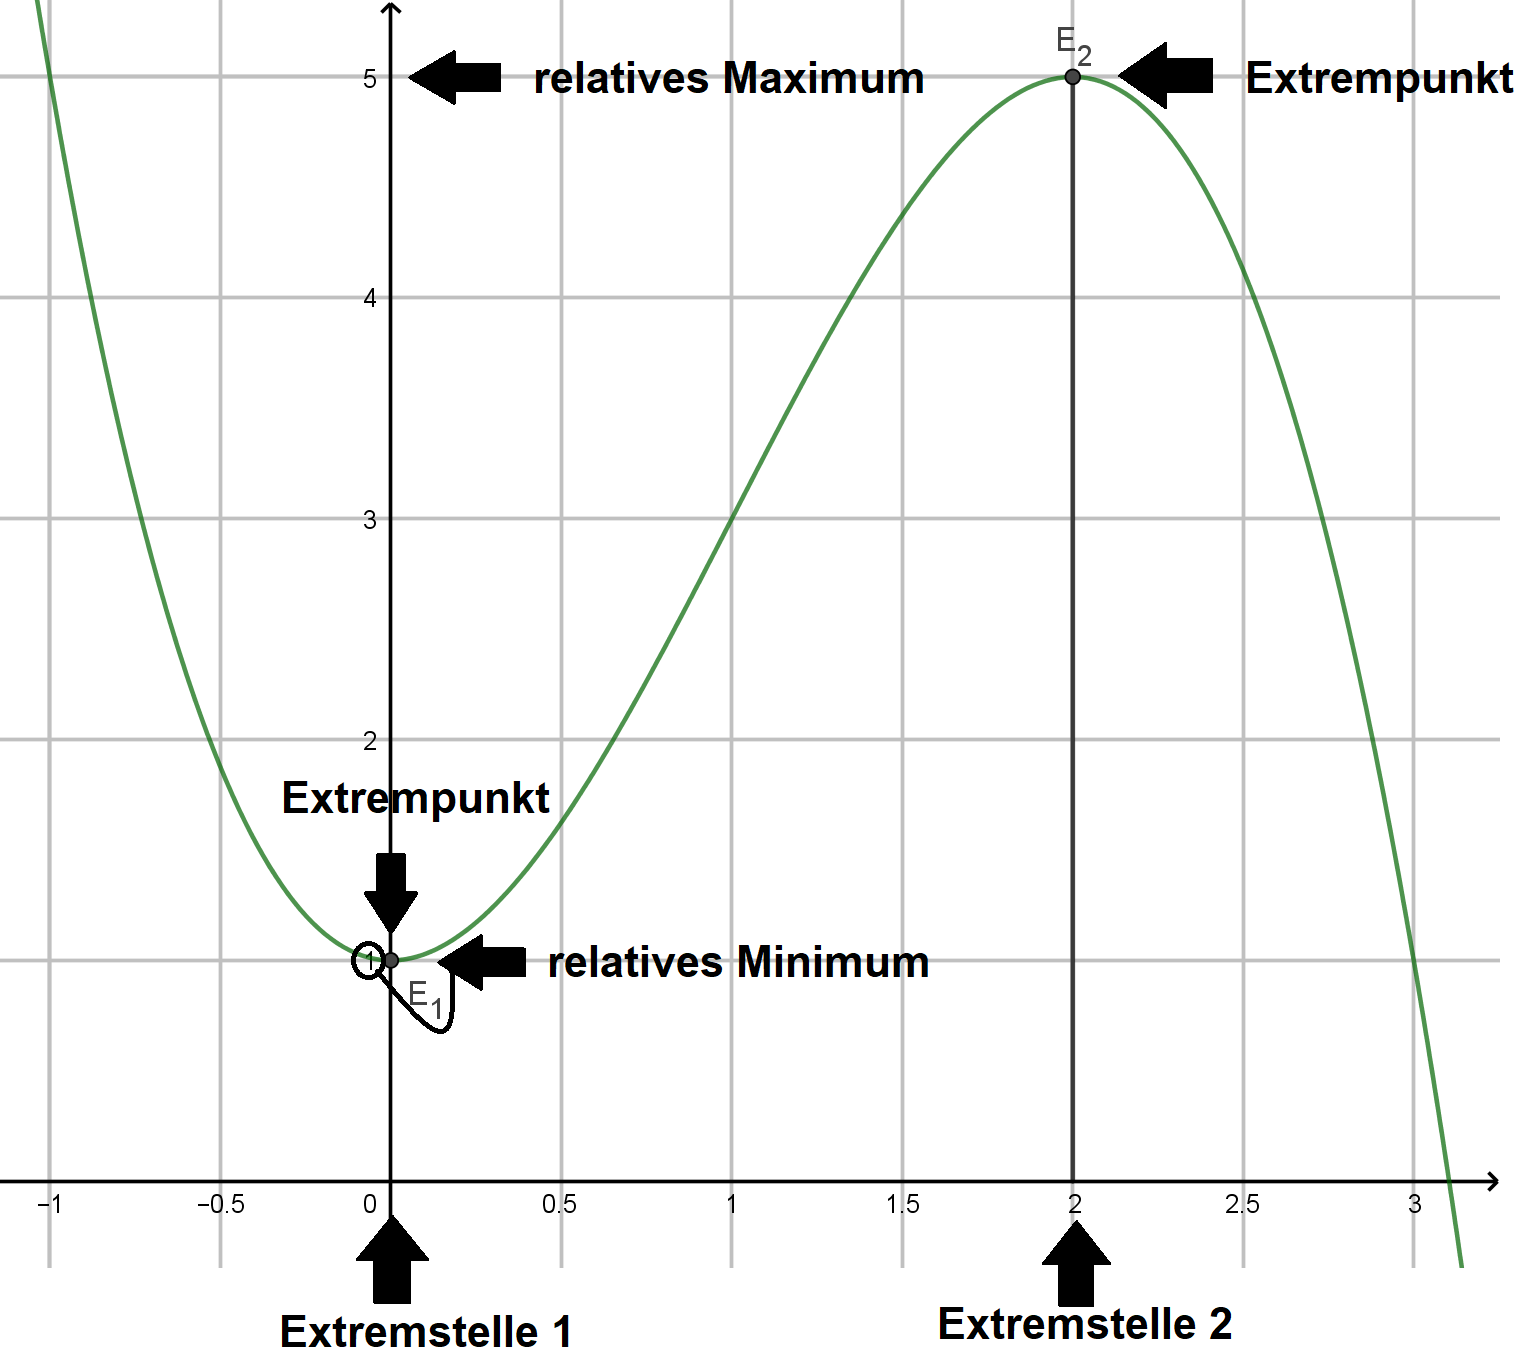
\includegraphics[width=0.48\textwidth]{../99_Bilder/042_Beg.png}
		\setcounter{section}{7}
		\setcounter{subsection}{3}
		\subsection{Extremstellen}
		Sollen wir den Graphen einer ganzrationalen Funktion \(f(x)\) zeichnen, benötigen wir zusätzlich zu den oben genannten Informationen noch weitere markante Stellen und die dazugehörigen Punkte.\\
		Die Rede ist von der \underline{\textbf{Extremstelle} \(\mathbf{x_{E}}\)}. Natürlich kann eine Funktion auch keine oder mehr als eine Extremstelle besitzen.\\
		\par\noindent
		Um diese zu bestimmen, benötigen wir die erste Ableitung \(f'(x)\) der Funktion.\\
		Wir erinnern uns daran, dass die Steigung des Funktionsgraphen am Hoch- bzw. Tiefpunkt 0 ist, also weder steigt noch fällt.\\
		\par\noindent
		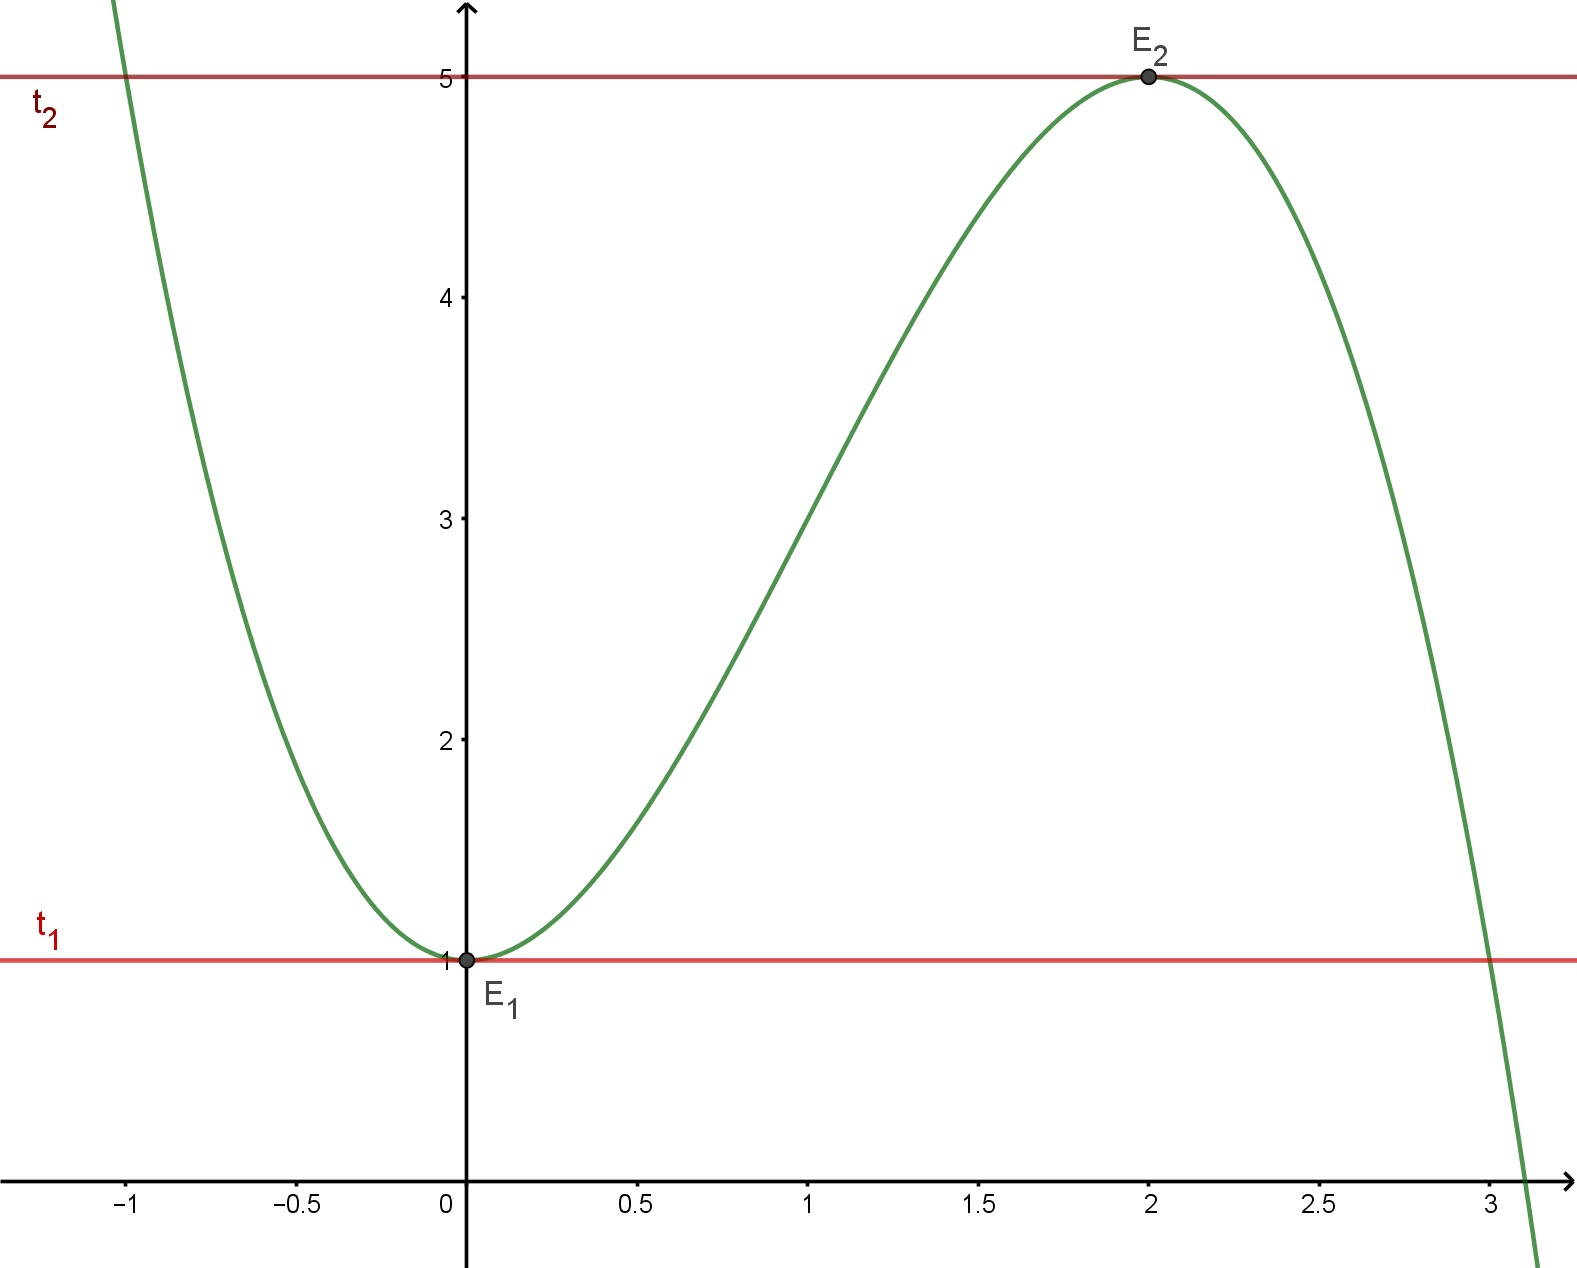
\includegraphics[width=0.48\textwidth]{../99_Bilder/042_EST_Tang.jpg}\\
		\par\noindent
		Die erste Ableitung \(\mathbf{f'(x)}\) entspricht der \textbf{Steigungsfunktion}.\\
		Um also herauszufinden, für welche \(x-Stellen\) die Funktion ein \textbf{relatives Maximum/Minimum} besitzt, bestimmen wir die \textbf{Nullstellen} der \textbf{ersten Ableitung}.\\
		\color{red}{\underline{Vorsicht!}}\normalcolor{} Zu beachten ist, die berechnete Nullstelle der ersten Ableitung ist nur dann eine Extremstelle, wenn die \textbf{zweite Ableitung} an dieser Stelle (also \(f''(x_E)\)) \underline{nicht} 0 it.
		\begin{framed}
			\noindent
			\(x_E\) ist eine Extremstelle von \(f(x)\), wenn
			\begin{itemize}[label=-]
				\item \textbf{notwendige Bedingung:}\\
				\(f'(x_E) = 0\)
			\end{itemize}
			und
			\begin{itemize}[label=-]
				\item  \textbf{hinreichende Bedingung:}\\
				\(f''(x_E) \neq 0\)
			\end{itemize}
		\end{framed}
		\noindent
		Haben wir die Extremstelle \(x_E\) bestimmt, setzen wir diese in die Ausgangsfunktion \(f(x)\) ein, um die x- und y-Koordinaten zu bestimmen.\\
		\par\noindent
		\textbf{Beispiel:} \(f(x) = x^3 + 0,5x^2 - 3,5x -3\)\\
		\par\noindent
		Zunächst bestimmen wir die erste Ableitung: \(f'(x) = 3x^2 + x - 3,5\)\\
		Anschließend die zweite Ableitung: \(f''(x) = 6x + 1\).\\
		\par\noindent
		Um nun die Nullstellen mit Hilfe der pq-Formel zu bestimmen, bringen wir die Funktion durch ausklammern in die entsprechende Form \(\Rightarrow f'(x) = 3(x^2+\underbrace{\frac{1}{3}}_{p}x\underbrace{-\frac{7}{6}}_{q})\).\\
		\begin{align*}
			x_{1/2} = -\frac{1}{6}\pm\sqrt{\left(\frac{1}{6}\right)^2 +\frac{7}{6}}\\
			x_{1/2} = -\frac{1}{6}\pm\sqrt{\frac{1}{36}+\frac{7}{6}}\\
			x_{1/2} = - \frac{1}{6}\pm\sqrt{\frac{43}{36}}\\
			\\
			x_1 = - \frac{1}{6}+\sqrt{\frac{43}{36}} = \frac{-1+\sqrt{43}}{6}\\
			x_2 = - \frac{1}{6}-\sqrt{\frac{43}{36}} = -\frac{1+\sqrt{43}}{6}
		\end{align*}
		Um sicher zu gehen, dass es sich hierbei auch wirklich um Extremstellen handelt, setzen wir die \(x\)-Stellen in die zweite Ableitung ein.\\
		\begin{align*}
			f''(x_1) & = 6\cdot{}\left(\frac{-1+\sqrt{43}}{6}\right) + 1\\
			& = -1+\sqrt{43} + 1 \neq 0\\
			\\
			f''(x_2) &=  6\cdot{}\left(-\frac{1+\sqrt{43}}{6}\right) + 1\\
			& = -1-\sqrt{43} + 1 \neq 0\\
		\end{align*}
		Bei \(x_1\) und \(x_2\) handelt es sich also offensichtlich um Extremstellen. Wir berechnen nun die dazugehörigen y-Koordinaten und erhalten so die Punkte.\\
		\begin{align*}
			f(x_1) & = (\frac{-1+\sqrt{43}}{6})^3 + 0,5\cdot\left(\frac{-1+\sqrt{43}}{6}\right)^2\\
			& -3,5\cdot\left(\frac{-1+\sqrt{43}}{6}\right) -3\\
			& = -5,02\\
			\\
			f(x_2) & = (-\frac{1+\sqrt{43}}{6})^3 + 0,5\cdot\left(-\frac{1+\sqrt{43}}{6}\right)^2\\
			& -3,5\cdot\left(-\frac{1+\sqrt{43}}{6}\right) -3\\
			& = 0,2
		\end{align*}
		Unsere Extrempunkte sind \(E_1(\frac{-1+\sqrt{43}}{6}|-5,02)\) und \(E_2(-\frac{1+\sqrt{43}}{6}|0,2)\).\\
	\end{worksheet}
\end{document}